\documentclass{article}

\usepackage{graphicx}
\usepackage{tikz}
\usepackage{tikzsymbols}
\usetikzlibrary{calc,patterns,shapes.geometric}
\pagestyle{empty}
\usepackage[margin=0pt]{geometry}
\geometry{papersize={14in,12in}}

\def\centerarc[#1](#2)(#3:#4:#5){\draw[#1] ($(#2)+({#5*cos(#3)},{#5*sin(#3)})$) arc (#3:#4:#5);}

\begin{document}
	\begin{figure}
		\centering
		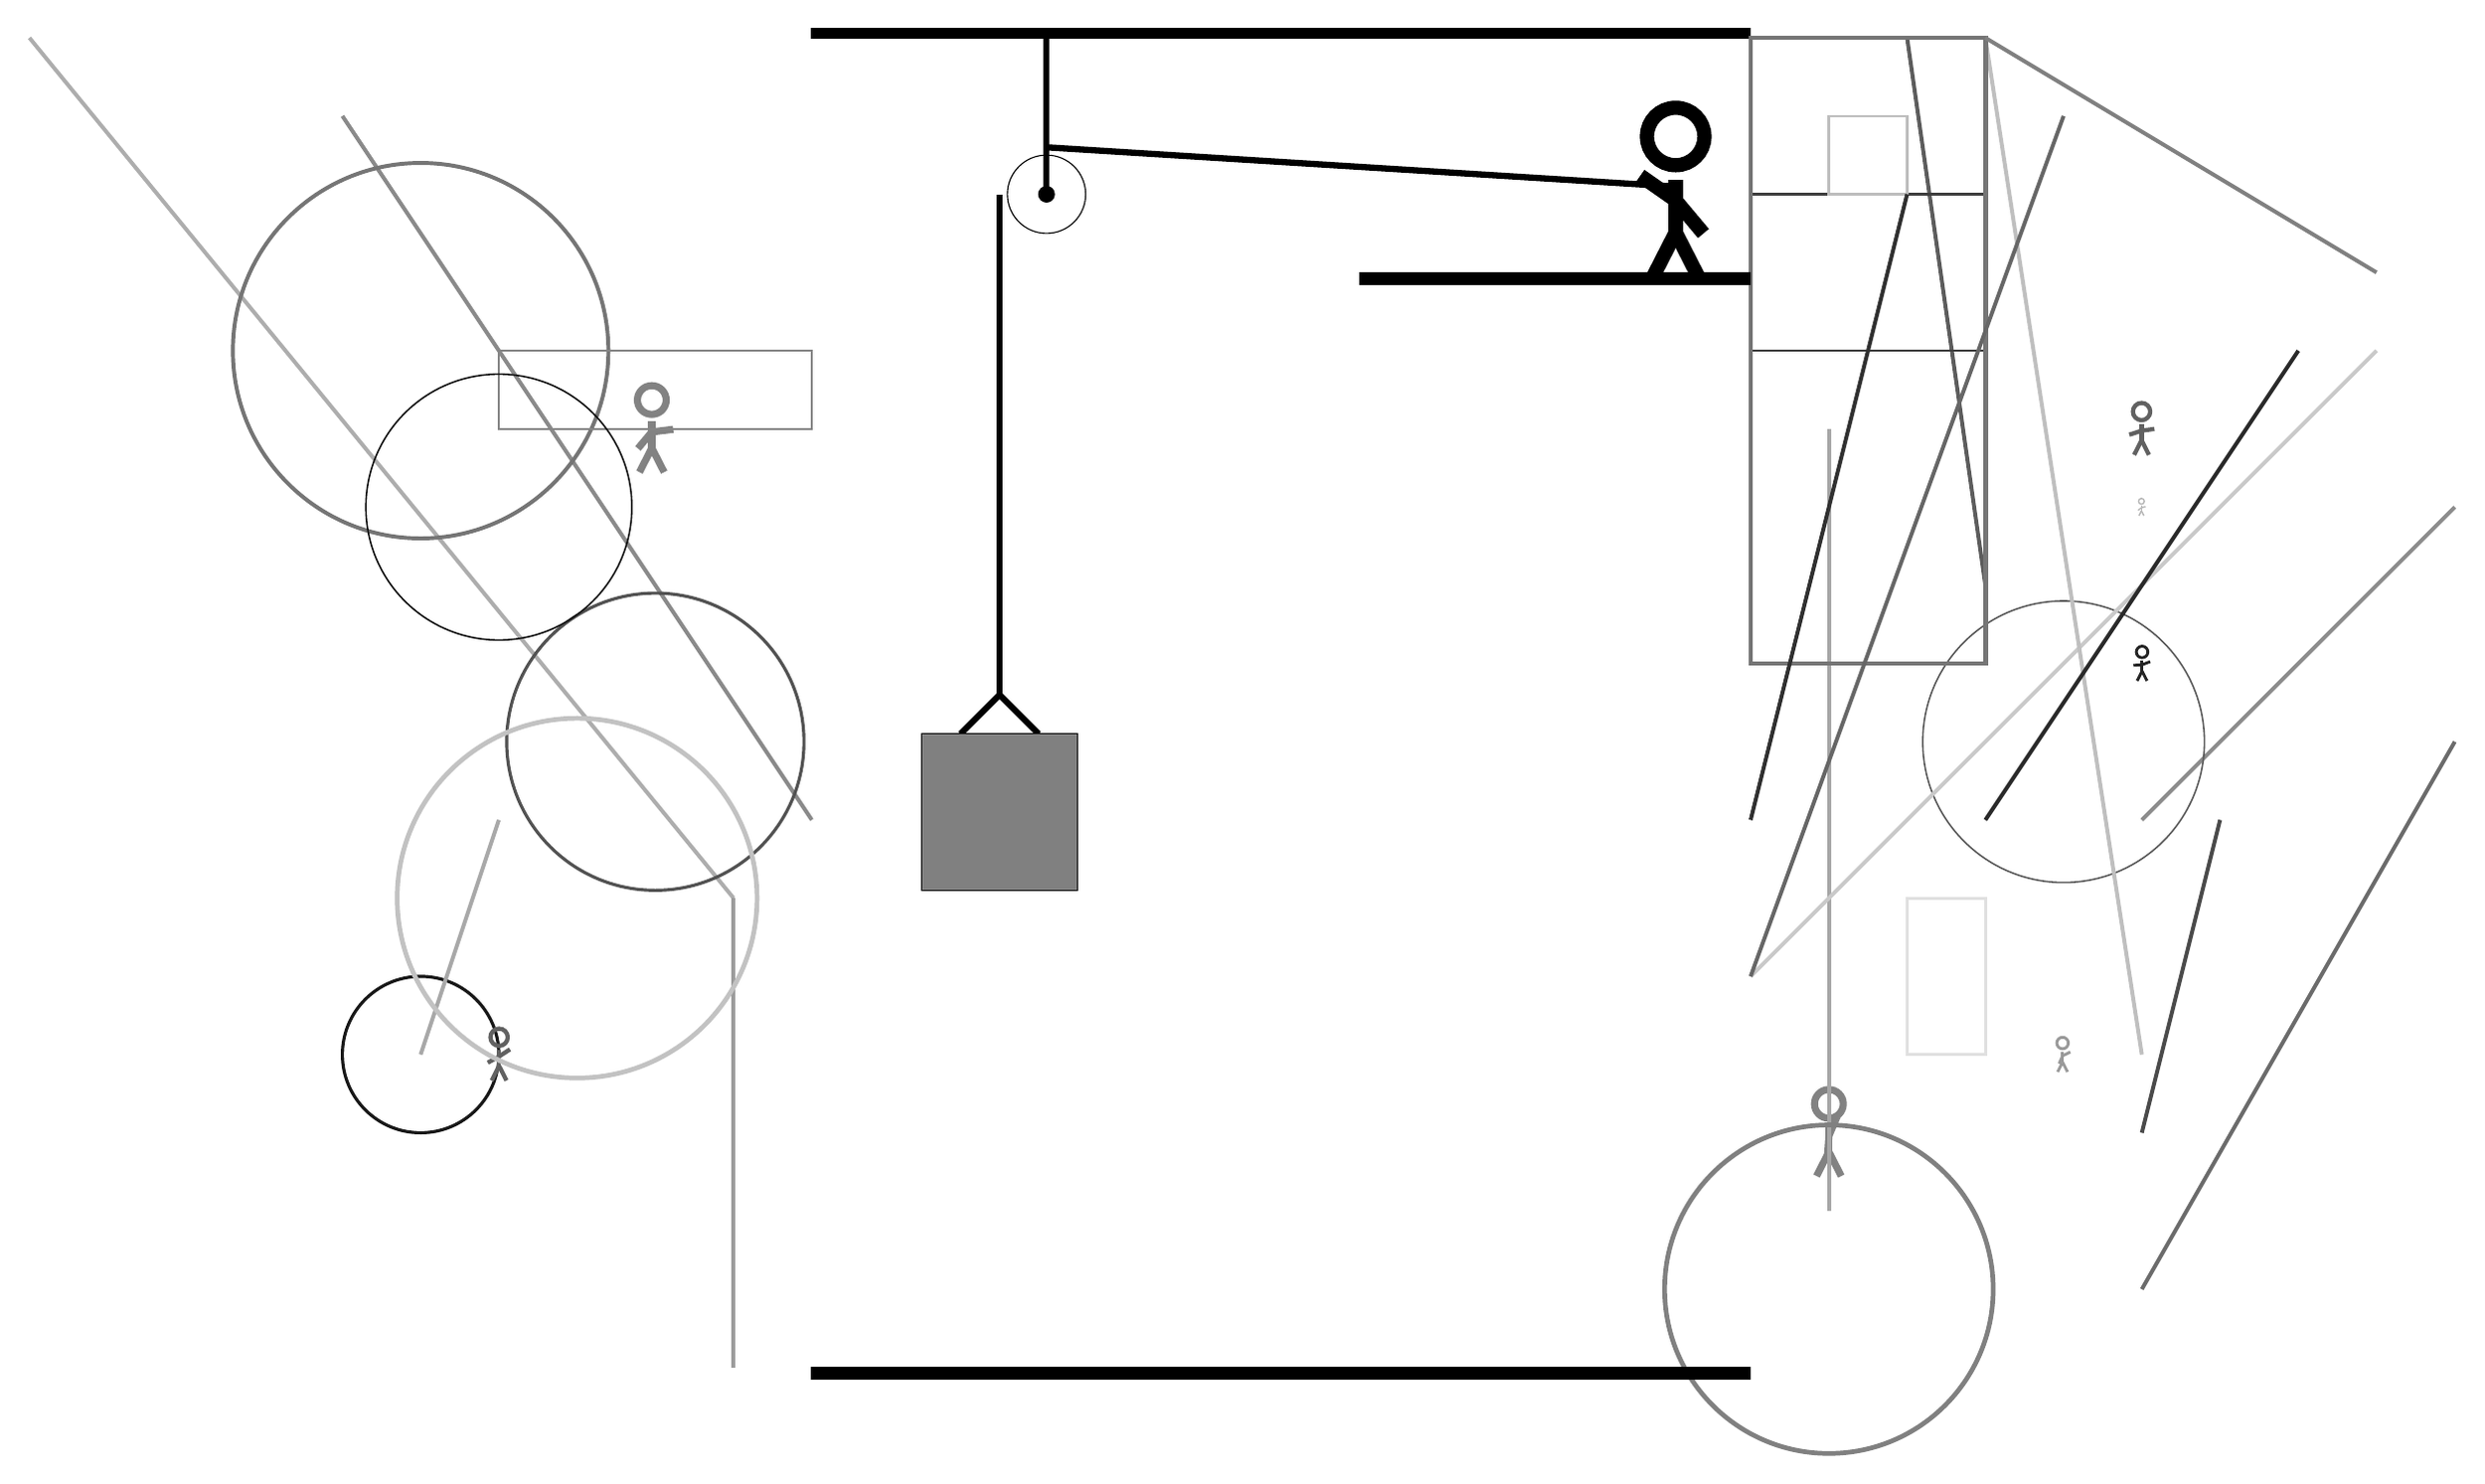
\begin{tikzpicture}
			%%%%% START %%%%%
			
			\draw[fill=black] (-2, 14) rectangle (10, 14.125);
			
			\draw (1, 12) circle (0.5);
			\draw[fill=black] (1, 12) circle (0.1);
			\draw[line width=0.8mm] (1, 14) -- (1, 12);
			
			\draw[line width=0.8mm](-0.1, 5.1) --  (0.4, 5.6) -- (0.9, 5.1);
			\draw[fill=black!50] (-0.6, 5.1) rectangle (1.4, 3.1);
			
			\draw[line width=0.5mm, color=black!32](-3, 3) -- (-12, 14);
			
			\draw[line width=0.5mm, color=black!45](15, 4) -- (19, 8);
			\node[line width=0.3mm, color=black!49] at (-4, 9) {\Strichmaxerl[5][50][7]};
			\draw[line width=0.5mm, color=black!71](15, 0) -- (16, 4);
			
			\draw[line width=0.5mm, color=black!46](-2, 4) -- (-8, 13);
			
			\node[line width=0.7mm, color=black!49] at (11, 0) {\Strichmaxerl[5][86][67]};
			\node[line width=0.4mm, color=black!28] at (15, 8) {\Strichmaxerl[1][38][15]};
			
			\node[line width=0.4mm, color=black!62] at (15, 9) {\Strichmaxerl[3][18][8]};
			\draw[line width=0.5mm, color=black!64](12, 14) -- (13, 7);
			\draw[line width=0.5mm, color=black!39](-3, 3) -- (-3, -3);
			\draw[line width=0.5mm, color=black!35] (11, 9) rectangle (11, -1);
			
			\node[line width=0.4mm, color=black!86] at (15, 6) {\Strichmaxerl[2][4][21]};
			\draw [line width=0.6mm, color=black!50](11, -2) circle (2.1);
			
			\draw [line width=0.5mm, color=black!54](-7, 10) circle (2.4);
			\draw [line width=0.4mm, color=black!91](-7, 1) circle (1.0);
			\draw[line width=0.5mm, color=black!34](-7, 1) -- (-6, 4);
			
			\draw [line width=0.7mm, color=black!77](-6, 8) circle (0.0);
			\draw [line width=0.2mm, color=black!65](14, 5) circle (1.8);
			\node[line width=0.3mm, color=black!62] at (-6, 1) {\Strichmaxerl[3][29][33]};
			\draw[line width=0.3mm, color=black!76] (10, 12) rectangle (13, 10);
			\draw[line width=0.2mm, color=black!48] (-2, 10) rectangle (-6, 9);
			
			\draw[line width=0.5mm, color=black!21](10, 2) -- (18, 10);
			\draw [line width=0.4mm, color=black!68](-4, 5) circle (1.9);
			\draw[line width=0.5mm, color=black!25](15, 1) -- (13, 14);
			\draw[line width=0.4mm, color=black!12] (12, 1) rectangle (13, 3);
			\draw [line width=0.6mm, color=black!24](-5, 3) circle (2.3);
			\draw[line width=0.6mm, color=black!54] (10, 6) rectangle (13, 14);
			\draw[line width=0.5mm, color=black!58](15, -2) -- (19, 5);
			\draw[line width=0.5mm, color=black!84](13, 4) -- (17, 10);
			\draw[line width=0.5mm, color=black!50](13, 14) -- (18, 11);
			\draw[line width=0.5mm, color=black!60](10, 2) -- (14, 13);
			
			\draw[line width=0.3mm, color=black!26] (11, 12) rectangle (12, 13);
			\draw [line width=0.2mm, color=black!94](-6, 8) circle (1.7);
			\draw[line width=0.5mm, color=black!81](12, 12) -- (10, 4);
			\node[line width=0.7mm, color=black!40] at (14, 1) {\Strichmaxerl[2][66][26]};
			
			\draw[line width=0.8mm](0.4, 12) -- (0.4, 5.6);
			\centerarc[line width=0.8mm](1, 12)(90:180:0.6)
			\draw[line width=0.8mm](1, 12.6) -- (9, 12.1);
			
			\node at (9, 12) {\Strichmaxerl[10][-35][-50]};
			\draw[fill=black] (5, 11) rectangle (10, 10.85);
			
			\draw[fill=black] (-2, -3) rectangle (10, -3.15);
			
			%%%%% END %%%%%
		\end{tikzpicture}
	\end{figure}	
\end{document}